% Latex template: https://github.com/mqTeXUsers/Macquarie-University-Beamer-Theme

% Slide Masters:

% Title
% Text
% 2 column
% Full-image
% Bibliography
% Closing
 
\documentclass[aspectratio=1610, 11pt]{beamer} % Aspect ratio
% https://tex.stackexchange.com/a/14339/5483 
% Possible values: 1610, 169, 149, 54, 43 and 32.
% 169 = 16:9

\PassOptionsToPackage{table}{xcolor}    %https://tex.stackexchange.com/a/5365/5483

\usetheme{macquarie}
\usepackage{multicol} % https://tex.stackexchange.com/a/396018/5483
\usepackage{xurl}
\usepackage[british]{babel}       % Set language
% \usepackage[utf8x]{inputenc}      % Set encoding
\usepackage{colortbl}
\mode<presentation>           % Set options
{
  \usetheme{default}          % Set theme
  \usecolortheme{default}         % Set colors
  \usefonttheme{default}          % Set font theme
  \setbeamertemplate{caption}[numbered] % Set caption to be numbered
}

% Uncomment this to have the outline at the beginning of each section highlighted.
%\AtBeginSection[]
%{
%  \begin{frame}{Outline}
%    \tableofcontents[currentsection]
%  \end{frame}
%}

\usepackage{graphicx}         % For including figures
\usepackage{booktabs}         % For table rules
\usepackage{hyperref}         % For cross-referencing


\usepackage{enumitem} % https://tex.stackexchange.com/a/2292/5483

%https://tex.stackexchange.com/a/371844/5483
\setbeamerfont{bibliography entry author}{size=\tiny}
\setbeamerfont{bibliography entry title}{size=\tiny}
\setbeamerfont{bibliography entry location}{size=\tiny}
\setbeamerfont{bibliography entry note}{size=\tiny}
\setbeamerfont{bibliography item}{size=\tiny}

%https://tex.stackexchange.com/q/333587/5483
%TODO SHAWN REPLACE OSF URL
%\setbeamertemplate{footline}{\strut~\texttt{https://github.com/MQ-FOAR705/MQ-FOAR705-Week1}\hfill\insertframenumber~/~\inserttotalframenumber\strut~~~}

\title{FOAR705 Week 4} % Presentation title
\author{Brian Ballsun-Stanton | Shawn A Ross | Kathryn Elliot}               % Presentation author
\institute{Faculty of Arts}         % Author affiliation
\date{Friday 23 August 2019}                 % Today's date  
\begin{document}

% Title page
% This page includes the informations defined earlier including title, author/s, affiliation/s and the date
% \begin{frame}[noframenumbering]

\maketitle

  
% \end{frame}

\begin{frame}{Today's Plan}
  \tableofcontents
\end{frame}

\section{Minute card reflection}
\begin{frame}{Assignment overview 1}

Most frequent red sticky note theme was: ``I'm not super clear on what tasks are necessary each week in some cases in relation to what we are marked on.'' 

In Cloudstor, Assignments, Week4Homework:

``Expectations:

You have two things to work on this week:

Work on: http://swcarpentry.github.io/shell-novice/ and do episodes: Introduction, Navigating Files and Directories, Working with Files. Put results into a new (or new section, or otherwise demarcate them) learning journal.

Finish Elaboration I. This is due in cloudstor only before the Week 5 class (though it will form part of your Elaboration II submission). Commit to git as you are committing all assignments, in whatever organisation you choose.''

\end{frame}

\begin{frame}{Assignment overview 2}

Focus on the assignments to meet expectations. Do readings if possible. 

Elaboration is assessable (combined parts I \& II). Worth 15\% of the proof of concept marks. 

Shell Learning Journal, due as Week 6 participatory task.

Copying the cloudstor Week$X$Homework documents to the week by week lines in iLearn. 

\end{frame}

\begin{frame}{Elaboration I}

{\small 
Using the step-by-step breakdown of your problems / solutions developed last week, identify technologies (programming languages, software libraries, APIs (Application programming interfaces, the means by which one program talks to another program) and other components of a modern data collection or processing workflow) that could accomplish each step. You may want to specify more than one possible technology. 

This document can be written in any format (though we encourage further practice in LaTeX) and should be as long as it needs to be. If you find yourself testing too many steps or technologies which depend on each other, you may wish to adjust your scope to be more specific. The judgement call for “too many” is “Can you see yourself learning enough to use and connect these tools and techniques in the next month?” 

Note: You will be testing these things for your next assignment (Elaboration II). Figure out the least work possible to get these things to fail your expectations. Plan alternate routes, assuming that most things will not work the way you expect them to. 

This elaboration planning document is due on Cloudstor by the start of class, week 5. You will use it as part of your graded Elaboration II submission, week 6.}

    
\end{frame}

\begin{frame}{Elaboration I advice}

Read the beginning of Chapter 7 in , through 'Elaboration and Iterations' (plus any subsequent sections where you think you need more detail).

The goal of the assignment is to:

\begin{itemize}[label=\textbullet]
    \item get a more detailed understanding of requirements;
    \item start charting ways to deliver those requirements;
    \item mitigate risk / de-scope as necessary (fail early and often);
    \item onfirm your earlier scoping analysis, ensuring that the tool or workflow you are developing does something you need.
\end{itemize}

The hardest part will probably be finding and choosing technologies. Doing so will likely require consultations with us. Please attend consultation hours and use Slack.

\end{frame}

\begin{frame}{Elaboration I examples}

\begin{itemize}[label=\textbullet]
    \item Social science: build a pipeline to get data from a public source (AURIN, ADA, data.gov.au, etc.) or from your own social surveys using an API and do something with that data (and then maybe resubmit the improved dataset if applicable).
    \item Ethnography / oral history: adapt an existing metadata capture mobile application to your needs.
    \item Textual or Media studies: build or adapt a system to manage metadata about the items in your corpus.
    \item Textual research: develop a text analysis tool using Voyant for your corpus.
    \item Archival research: build a pipeline around the management of your archival sources (e.g., photographs of them) using Zotero, Tropy, or other open-source tools.
    \item Cross-disciplinary: develop a full-service, redeployable bibliography management pipeline around one of the open managers (e.g., Zotero) for your thesis; develop a redeployable TeX pipeline / template for your thesis. 
\end{itemize}

The hardest part will probably be finding and choosing technologies. Doing so will likely require consultations with us. Please attend consultation hours and use Slack.

\end{frame}

\section{Software Carpentry: Shell}

\begin{frame}{Setup}

Installing the shell:

{\tt https://swcarpentry.github.io/shell-novice/setup.html}

Mac users, go into spotlight, launch terminal.

Windows users download Git For Windows from {\tt https://gitforwindows.org/}

(other methods out of scope for today, ask during consultation)
\end{frame}

\begin{frame}{Background}

At a high level, computers do four things:
\begin{itemize}[label=\textbullet]
    \item run programs
    \item store data
    \item communicate with each other, and
    \item interact with us
\end{itemize}


\end{frame}

\begin{frame}{Graphic User Interface}
    
   The Graphic User Interface (GUI): Mouse, windows, `drag and drop'. `Knowledge-in-the- world'. \cite{Norman2013-xk}
    \begin{figure}[H]
        
        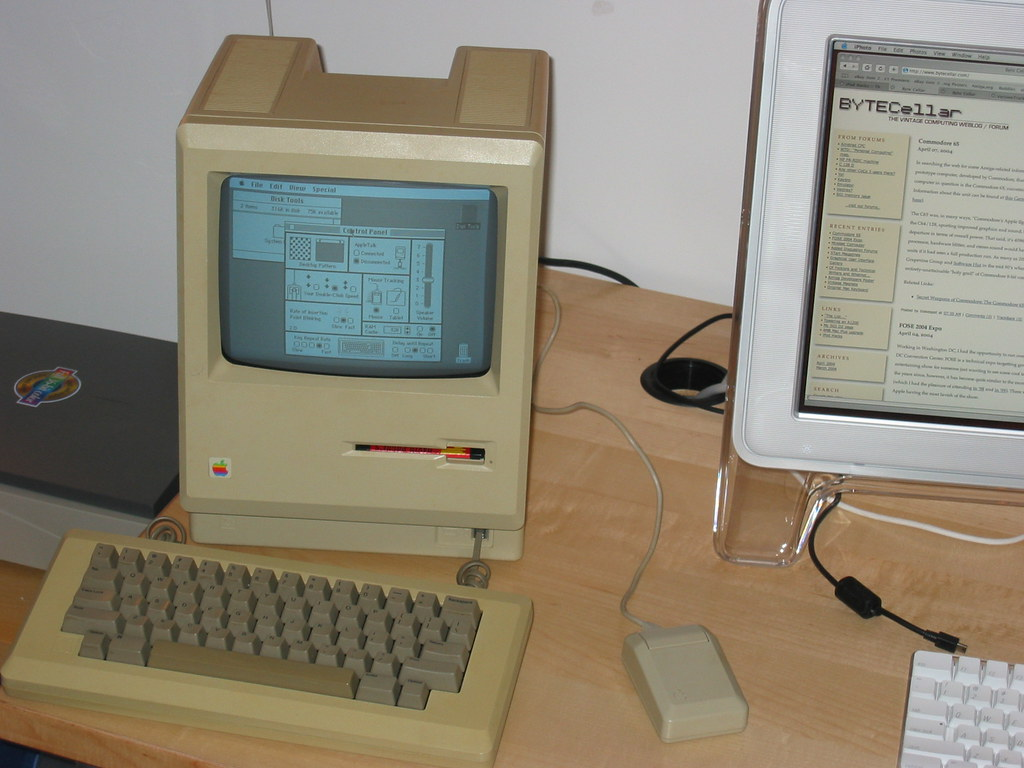
\includegraphics[width=0.6\textwidth]{figures/2388811229_7e3a50354d_b_d.jpg}
        \caption{Blake Patterson https://flic.kr/p/4D6hmv CC-By}
        \label{fig:gui}
    \end{figure}
   
\end{frame}

\begin{frame}{Command Line Interface}

    The Command Line Interface (CLI): Empty screen with a {\tt \$}. `Knowledge-in-the-head'\cite{Norman2013-xk}. Type instructions and computer executes quickly.

`The teletype would send that line to
the computer, which might or might not respond with some lines of its own, which the
teletype would hammer out–producing, over time, a transcript of your exchange with
the machine...' \cite{Stephenson1999-fw}

    
     \begin{figure}[H]

     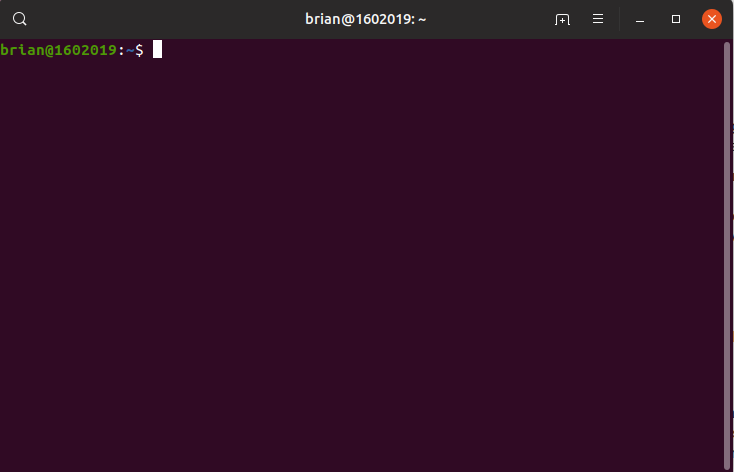
\includegraphics[width=.3\textwidth]{figures/terminal.png}
        \caption{Brian Ballsun-Stanton. CC0}
        \label{fig:cli}
        \end{figure}

\end{frame}
\begin{frame}{SWC ls and prompt}

Let us look at the prompt now...
\end{frame}

\begin{frame}{Nelle's Pipeline}

Nelle Nemo, a marine biologist, has just returned from a six-month survey of the North Pacific Gyre, where she has been sampling gelatinous marine life in the Great Pacific Garbage Patch. She has 1520 samples in all and now needs to:
\begin{enumerate}[label=\arabic*)]
    \item Run each sample through an assay machine that will measure the relative abundance of 300 different proteins. The machine’s output for a single sample is a file with one line for each protein.
    \item Calculate statistics for each of the proteins separately using a program her supervisor wrote called goostats.
    \item Write up results. Her supervisor would really like her to do this by the end of the month so that her paper can appear in an upcoming special issue of Aquatic Goo Letters.
\end{enumerate}

Two weeks to run 1520 samples.     

Using GUI would take 1520 different file selections. Finishing analysis would take longer than the month available.


As a bonus, once she has put a processing pipeline together, she will be able to use it again whenever she collects more data.
\end{frame}

\begin{frame}{Navigating files and directories}

Episode 2, Navigating Files and Directories:

How can I move around on my computer? 

How can I see what files and directories I have? 

How can I specify the location of a file or directory on my computer?

\end{frame}

\section{Minute cards!}
\begin{frame}{Feedback time}

On your green sticky, write one thing we did well today.

On your red sticky, write one thing we could improve upon for next time. Be specific. 

\end{frame}

\section{References}

\begin{multicols}{2}[]
\bibliography{references}
\bibliographystyle{apalike}
\end{multicols}


% \begin{frame}[allowframebreaks]{References}
  
%   \bibliography{references}
%   \bibliographystyle{apalike}
% \end{frame}


\begin{frame}{Thank you!}

% This presentation is available at:
% \texttt{https://osf.io/...}

Source code for this presentation is available at: \url{https://github.com/MQ-FOAR705/MQ-FOAR705-Week3}

This work is licensed under a Creative Commons Attribution 4.0 International License.

\end{frame}



\end{document}